\chapter{Software Requirement Specifications}
\label{ch:srs}

AetherFlow is intended to help developers use local and cloud language models through one gateway. This chapter sets out what the gateway must do, how developers and administrators will interact with it, and the conditions under which it is expected to operate. It also describes the proposed interfaces, storage design, and main operational risks. The numerical requirements below are acceptance targets for testing; they are not presented as measurements of a completed deployment.

\section{List of Features}
\label{sec:list-of-features}

The proposed system has twelve main features. Together, they cover the path from a request in the editor to the delivery and recording of its response.

\begin{enumerate}
    \item \textbf{Editor context capture:} The extension collects the selected code, cursor position, language, and relevant project paths so that a request includes the context needed for the chosen action.
    \item \textbf{Credential screening:} The gateway checks incoming content for passwords, API keys, and private-key material before contacting a model provider.
    \item \textbf{Personal-data masking:} Detected personal values are replaced with placeholders. A protected temporary mapping allows the gateway to restore those values in the response.
    \item \textbf{Local processing rules:} Requests containing credentials or otherwise classified as confidential are restricted to approved internal backends. A lower price or higher quality estimate cannot override this restriction.
    \item \textbf{Two-stage cache checking:} Vector search finds related requests, after which a second check assesses whether a stored answer is suitable for reuse.
    \item \textbf{Cached responses:} A verified answer can be returned without another generation call. The target response time is defined in NFR-02.
    \item \textbf{Quality prediction:} For a cache miss, the gateway estimates how well each candidate model is likely to answer before requesting a completion.
    \item \textbf{Model selection:} The policy engine compares predicted quality, estimated cost, and recent response times among eligible backends.
    \item \textbf{Service monitoring:} Health checks and rolling latency measurements help the gateway avoid unavailable or slow services.
    \item \textbf{Failure recovery:} Circuit breakers limit repeated calls to failing providers. Where possible, the gateway retries through an eligible local model and reports the outcome to the client.
    \item \textbf{Administrative controls:} Authorized administrators can adjust routing priorities, endpoint settings, and department quotas through a dashboard.
    \item \textbf{Audit records:} An append-only trail records request identifiers, prompt hashes, detection counts, masking actions, and routing outcomes. Integrity checks must make unauthorized changes detectable without storing the detected secrets themselves.
\end{enumerate}

\section{Functional Requirements}
\label{sec:functional-reqs}

The requirements are grouped by the part of the system responsible for them. The identifiers provide a consistent reference for implementation and acceptance testing.

\subsection{Functional Requirements for Developer Client}
\begin{itemize}
    \item \textbf{FR-01 (Context Ingestion):} When a developer starts a code action, the extension shall collect the selected text, active language, and relevant workspace information.
    \item \textbf{FR-02 (Payload Dispatch):} The client shall package the request as an OpenAI-compatible JSON completion payload and submit it asynchronously over a TLS connection.
    \item \textbf{FR-03 (Token Stream Rendering):} The client shall consume Server-Sent Events (SSE), display the response as it arrives, and render markdown and highlighted code without blocking the editor interface.
    \item \textbf{FR-04 (Execution Telemetry Display):} After a request finishes, the client shall provide an optional status view showing the serving category (cache, local, or cloud), elapsed time, and estimated savings against the configured cost baseline.
\end{itemize}

\subsection{Functional Requirements for Enterprise Administrator}
\begin{itemize}
    \item \textbf{FR-05 (Dynamic Routing Weights):} Authorized administrators shall be able to update quality, cost, and latency weights while the gateway is running. Workers shall apply a validated policy version to subsequent decisions without requiring a restart.
    \item \textbf{FR-06 (Model Registry Controls):} Administrators shall be able to add, edit, and remove endpoint registrations, manage their authentication settings, and record input and output token prices.
    \item \textbf{FR-07 (Quota Limits by Department):} The dashboard shall show daily and monthly token consumption by department. Once a configured cloud allowance is exhausted, further paid requests shall be blocked and an eligible local backend used where available.
    \item \textbf{FR-08 (Audit Logs Viewer):} Authorized administrators shall be able to search and export records of sensitive-data detections, token-vault operations, and routing decisions. The viewer shall expose event metadata rather than raw sensitive values.
\end{itemize}

\subsection{Functional Requirements for Gateway Core and Router}
\begin{itemize}
    \item \textbf{FR-09 (Input Privacy Screening):} The gateway shall check every request for credentials and personal information before cache lookup or model execution.
    \item \textbf{FR-10 (Hard Data Residency Enforcement):} The gateway shall exclude external providers whenever a request contains credentials or is classified as confidential. Masking shall not remove an existing local-only restriction.
    \item \textbf{FR-11 (Two-Tier Cache Verification):} The gateway shall retrieve cache candidates through vector search and verify a candidate before returning its answer. Reuse shall also respect the request's access scope and privacy policy.
    \item \textbf{FR-12 (Multi-Objective Model Selection):} Following a cache miss, the gateway shall score eligible backends and stream a response from the selected model. If no backend is eligible and available, it shall return a controlled failure rather than bypass the policy.
\end{itemize}

\section{Quality Attributes}
\label{sec:quality-attributes}

These attributes describe how the system should behave beyond completing its individual functions.
\begin{itemize}
    \item \textbf{Reliability:} Provider failures should be contained within the request-handling path. A circuit breaker should prevent repeated attempts against an unavailable service, and recovery should use only policy-compliant backends. If a stream has already started, the client should receive an explicit interruption or retry indication.
    \item \textbf{Extensibility:} Adding an endpoint that follows a supported protocol should require configuration changes rather than a gateway rebuild. A provider with a different protocol may require a separate adapter.
    \item \textbf{Security:} Connections between the client, gateway, and backends should use TLS~1.3. Placeholder mappings should remain in protected temporary storage and be removed when the request is complete or expires.
    \item \textbf{Modularity:} Privacy screening, caching, prediction, routing, and serving should communicate through typed interfaces so that one component can be tested or replaced without rewriting the others.
    \item \textbf{Usability:} Developers should be able to invoke assistance through familiar editor menus and shortcuts. Once the extension and connection settings are provisioned, routine actions should require little additional setup.
    \item \textbf{Interoperability:} The gateway should implement the supported OpenAI-compatible completion interface. Compatible clients should be able to use it by changing their endpoint and authentication settings.
\end{itemize}

\section{Non-Functional Requirements}
\label{sec:non-functional-reqs}

Acceptance tests must state the hardware, prompt lengths, model configuration, and load used. Here, p95 denotes the time within which 95\% of measured requests complete the specified operation.
\begin{itemize}
    \item \textbf{NFR-01 (Gateway routing delay):} At 100 requests per second, the target p95 overhead on a cache miss shall be no more than 15\,ms. This includes privacy screening, attempted cache lookup and verification, quality prediction, and policy selection, but excludes backend generation and client network time.
    \item \textbf{NFR-02 (Cache hit time):} A verified cache hit shall have a target p95 client round-trip time below 200\,ms under the agreed test conditions.
    \item \textbf{NFR-03 (Concurrent streams):} Each gateway node shall support at least 500 simultaneous streaming connections. Load tests shall check connection failures, response delay, and backpressure while this concurrency is maintained.
    \item \textbf{NFR-04 (Privacy key recall):} Screening shall detect every supported credential example in the acceptance dataset, including standardized API tokens, private keys, and database secrets. Results shall report missed detections as well as false alarms; success on this dataset does not imply detection of every possible secret format.
    \item \textbf{NFR-05 (Service uptime):} The deployment shall target at least 99.9\% availability over the agreed monitoring period, supported by redundant gateway instances and appropriate health checks.
    \item \textbf{NFR-06 (Memory use):} The gateway core and its helper models shall target less than 4\,GB of system RAM. This budget excludes the separate database services and the language-model serving processes.
\end{itemize}

\section{Assumptions}
\label{sec:assumptions}

The requirements rely on the following deployment conditions:
\begin{enumerate}
    \item \textbf{Controlled network boundary:} The gateway and approved local inference services run within an organization-controlled intranet or private network. Firewall and access rules define this trusted boundary.
    \item \textbf{Suitable inference hardware:} At least one local host has enough GPU memory for the selected 8B model, its precision, and the intended context length. Weight storage alone is not the complete memory requirement.
    \item \textbf{Authorized provider access:} Teams using cloud models have valid API credentials, and the deployment permits outbound HTTPS connections to approved endpoints.
    \item \textbf{Streaming support:} Clients support HTTP/1.1 or HTTP/2 and can process SSE responses incrementally.
    \item \textbf{Readable inputs:} The initial scope covers UTF-8 text prompts. Detecting secrets concealed through encryption, steganography, or unsupported input formats is outside this assumption.
\end{enumerate}

\section{Use Cases}
\label{sec:use-cases}

The four use cases describe the expected interaction between users and the gateway. Each records the starting conditions, the normal sequence, and an alternative outcome. Timing figures are test targets rather than example measurements.

Table~\ref{tab:uc01} follows a request from the editor to the returned answer.
\begin{table}[H]
\centering\small
\caption{Use Case UC-01: Query Execution through the Gateway}
\label{tab:uc01}
\renewcommand{\arraystretch}{1.08}
\begin{tabularx}{\textwidth}{|p{3.1cm}|X|}
\hline
\textbf{Name} & UC-01: End-to-End Query Execution via Gateway \\ \hline
\textbf{Actors} & Developer, editor extension, gateway, and model provider. \\ \hline
\textbf{Summary} & The developer requests assistance. The gateway checks privacy and cache eligibility, then returns a stored answer or selects a model. \\ \hline
\textbf{Preconditions} & Gateway reachable at its configured address (port 8000 by default); valid client token; an eligible backend available. \\ \hline
\textbf{Postconditions} & The editor receives an answer or a clear failure status, and the gateway records execution metrics. \\ \hline
\textbf{Special requirements} & Target completion time below 1.5\,s for the defined short-response workload; an eligible local fallback on provider timeout. \\ \hline
\textbf{Main flow} & 1. The developer invokes a code action.\newline 2. The extension sends the context over HTTPS.\newline 3. The gateway screens the request and checks the cache.\newline 4. On a miss, it selects an eligible backend.\newline 5. The client renders the streamed answer and displays telemetry. \\ \hline
\textbf{Alternative flow} & A verified cache match is returned without generation, subject to NFR-02. If no eligible backend remains, the client receives an explanatory error. \\ \hline
\end{tabularx}
\end{table}

Table~\ref{tab:uc02} describes a request containing information that must remain inside the organization.
\begin{table}[H]
\centering\small
\caption{Use Case UC-02: Privacy Screening and Local-Only Processing}
\label{tab:uc02}
\renewcommand{\arraystretch}{1.08}
\begin{tabularx}{\textwidth}{|p{3.1cm}|X|}
\hline
\textbf{Name} & UC-02: Automated Privacy Screening and Local Invariance \\ \hline
\textbf{Actors} & Developer, Privacy Analyzer, gateway, and local model service. \\ \hline
\textbf{Summary} & Screening identifies a credential in submitted code, and the gateway excludes external inference services. \\ \hline
\textbf{Preconditions} & Screening rules loaded; an approved local model operational. \\ \hline
\textbf{Postconditions} & Request content is processed within the approved boundary; the audit record identifies the applied restriction. \\ \hline
\textbf{Special requirements} & No request content sent to an external backend; screening target at most 10\,ms within the overall NFR-01 budget. \\ \hline
\textbf{Main flow} & 1. The developer submits code containing an API key.\newline 2. The gateway receives it over TLS.\newline 3. The Privacy Analyzer identifies the credential.\newline 4. The policy engine excludes cloud models.\newline 5. A local model responds, and the client displays the local routing decision. \\ \hline
\textbf{Alternative flow} & For maskable personal data, the gateway creates placeholders and restores them on return. Cloud processing is considered only if the sanitized request is permitted by policy and no local-only restriction applies. \\ \hline
\end{tabularx}
\end{table}

Table~\ref{tab:uc03} uses opposite code operations to illustrate why a nearby vector match may still be unsuitable.
\begin{table}[H]
\centering\small
\caption{Use Case UC-03: Cache Verification for Conflicting Requests}
\label{tab:uc03}
\renewcommand{\arraystretch}{1.08}
\begin{tabularx}{\textwidth}{|p{3.1cm}|X|}
\hline
\textbf{Name} & UC-03: Two-Tier Semantic Cache Verification and Inversion Rejection \\ \hline
\textbf{Actors} & Developer, semantic cache service, and vector database. \\ \hline
\textbf{Summary} & A decryption request retrieves an encryption example. The verifier rejects reuse because the requested operations differ. \\ \hline
\textbf{Preconditions} & The test cache contains the conflicting example; thresholds are calibrated on separate validation data. \\ \hline
\textbf{Postconditions} & The unsuitable entry is rejected and the request continues to model selection. \\ \hline
\textbf{Special requirements} & Target rejection rate above 99\% on the defined inversion test set. Cache processing must fit within NFR-01 when verification ends in a miss. \\ \hline
\textbf{Main flow} & 1. The developer requests decryption code.\newline 2. The bi-encoder represents the prompt as a vector.\newline 3. Retrieval returns a similar encryption request.\newline 4. The second gate assesses the pair and rejects reuse.\newline 5. The gateway selects a model to produce a fresh answer. \\ \hline
\textbf{Alternative flow} & If both gates accept a compatible request and its cache scope is valid, the gateway returns the saved answer within the NFR-02 target. \\ \hline
\end{tabularx}
\end{table}

Table~\ref{tab:uc04} describes a policy update during normal operation. Increasing the cost weight favours lower-cost choices, but does not force local routing unless a separate quota or privacy rule requires it.
\begin{table}[H]
\centering\small
\caption{Use Case UC-04: Updating Routing Priorities}
\label{tab:uc04}
\renewcommand{\arraystretch}{1.08}
\begin{tabularx}{\textwidth}{|p{3.1cm}|X|}
\hline
\textbf{Name} & UC-04: Dynamic Operational Policy Weight Tuning \\ \hline
\textbf{Actors} & Authorized administrator, dashboard, and policy engine. \\ \hline
\textbf{Summary} & The administrator increases the emphasis on cost as the billing period ends. Subsequent requests use the updated weights. \\ \hline
\textbf{Preconditions} & Administrator authenticated; gateway operating with a valid policy. \\ \hline
\textbf{Postconditions} & A validated policy version becomes active without restarting the gateway. \\ \hline
\textbf{Special requirements} & Each weight lies in $[0,1]$ and $w_q+w_c+w_l=1$; updates are applied atomically. \\ \hline
\textbf{Main flow} & 1. The administrator opens policy settings.\newline 2. The dashboard shows the current weights.\newline 3. The administrator edits and submits them.\newline 4. The server validates and publishes the new policy.\newline 5. Workers use it for subsequent routing decisions. \\ \hline
\textbf{Alternative flow} & Invalid weights are rejected with a clear explanation. The previous policy remains active until a valid update is accepted. \\ \hline
\end{tabularx}
\end{table}
\clearpage

\section{Hardware and Software Requirements}
\label{sec:hardware-software-reqs}

\subsection{Hardware Requirements}
\label{subsec:hardware-reqs}

Table~\ref{tab:hardware_specs} gives planning configurations for development and deployment. Final capacity depends on the selected models, quantization, context lengths, cache size, and request load.
\begin{table}[H]
\centering\small
\begin{tabularx}{\textwidth}{|p{2.4cm}|X|X|}
\hline
\textbf{Component} & \textbf{Development configuration} & \textbf{Production configuration} \\ \hline
Processor & 8-core x86-64 CPU, such as a Core i7 or Ryzen 7 & Server CPU with at least 16 cores, such as EPYC or Xeon \\ \hline
System memory & 16\,GB DDR4/DDR5 RAM & 64\,GB ECC RAM as an initial capacity plan \\ \hline
GPU & GPU with about 12\,GB VRAM for a suitable quantized model & A100 with 40/80\,GB VRAM, or two RTX 4090 cards where the serving setup supports them \\ \hline
Storage & 512\,GB NVMe SSD; planning read rate at least 3{,}000\,MB/s & 2\,TB enterprise PCIe Gen4 NVMe storage with suitable redundancy \\ \hline
Network & 100\,Mbps Ethernet or Wi-Fi for development & 10\,Gbps internal networking where the deployment requires it \\ \hline
\end{tabularx}
\caption{Proposed Development and Production Hardware}
\label{tab:hardware_specs}
\end{table}

\begin{itemize}
    \item \textbf{CPU capacity:} Asynchronous I/O helps while the gateway waits for services, but does not remove the computation needed for entity recognition, embeddings, and verification. Worker sizing must account for these tasks and their queues.
    \item \textbf{System memory:} The development allocation is intended for a modest database, vector collection, and helper-model workload. Production memory must be sized from measured use, especially when several workers hold their own model copies.
    \item \textbf{GPU memory:} Eight billion parameters at two bytes each require roughly 16\,GB for weights alone. The serving engine also needs memory for attention state and execution buffers. Quantization can reduce weight storage, but a 12\,GB configuration must still be tested with the intended model and context length.
    \item \textbf{Storage performance:} NVMe storage supports model loading and database activity. Throughput above 3{,}500\,MB/s is a preferred planning target, although sustained database performance also depends on access patterns and durability settings.
\end{itemize}

\subsection{Software Requirements}
\label{subsec:software-reqs}

The proposed stack separates the gateway, persistence services, model servers, and editor extension. The versions below describe the report's implementation baseline; the deployment must pin and test a compatible set rather than assume that every later release is interchangeable.
\begin{itemize}
    \item \textbf{Operating systems:} Ubuntu 22.04 or 24.04 LTS for servers; Windows 11 with WSL2 for development; macOS on Apple Silicon with Ollama for local experiments.
    \item \textbf{Runtimes and containers:} Python 3.11 for the gateway; Node.js and npm for the extension build, with Node.js 18 as the original baseline; Docker Engine 24 and Compose v2 for service deployment.
    \item \textbf{Storage services:} PostgreSQL 15 or 16 for relational records, Qdrant 1.9 for vector indexing, and Redis 7 for shared counters and latency buffers.
    \item \textbf{Model tooling:} vLLM 0.5 or Ollama 0.3 for inference; Presidio 2.2 for sensitive-data processing; Transformers 4.40, Sentence-Transformers 3.0, and ONNX Runtime 1.18 for the helper models where supported.
    \item \textbf{Gateway libraries:} FastAPI 0.111 with Uvicorn workers, HTTPX 0.27 for asynchronous service calls, and Pydantic v2 for request validation.
    \item \textbf{Editor tooling:} Visual Studio Code 1.85 and TypeScript 5 form the original extension development baseline.
\end{itemize}

\section{Graphical User Interface}
\label{sec:gui}

Developers interact with AetherFlow through a VS Code extension, while administrators use a web dashboard. Figure~\ref{fig:gui_mockups} shows the proposed layout of each interface.
\begin{figure}[H]
\centering
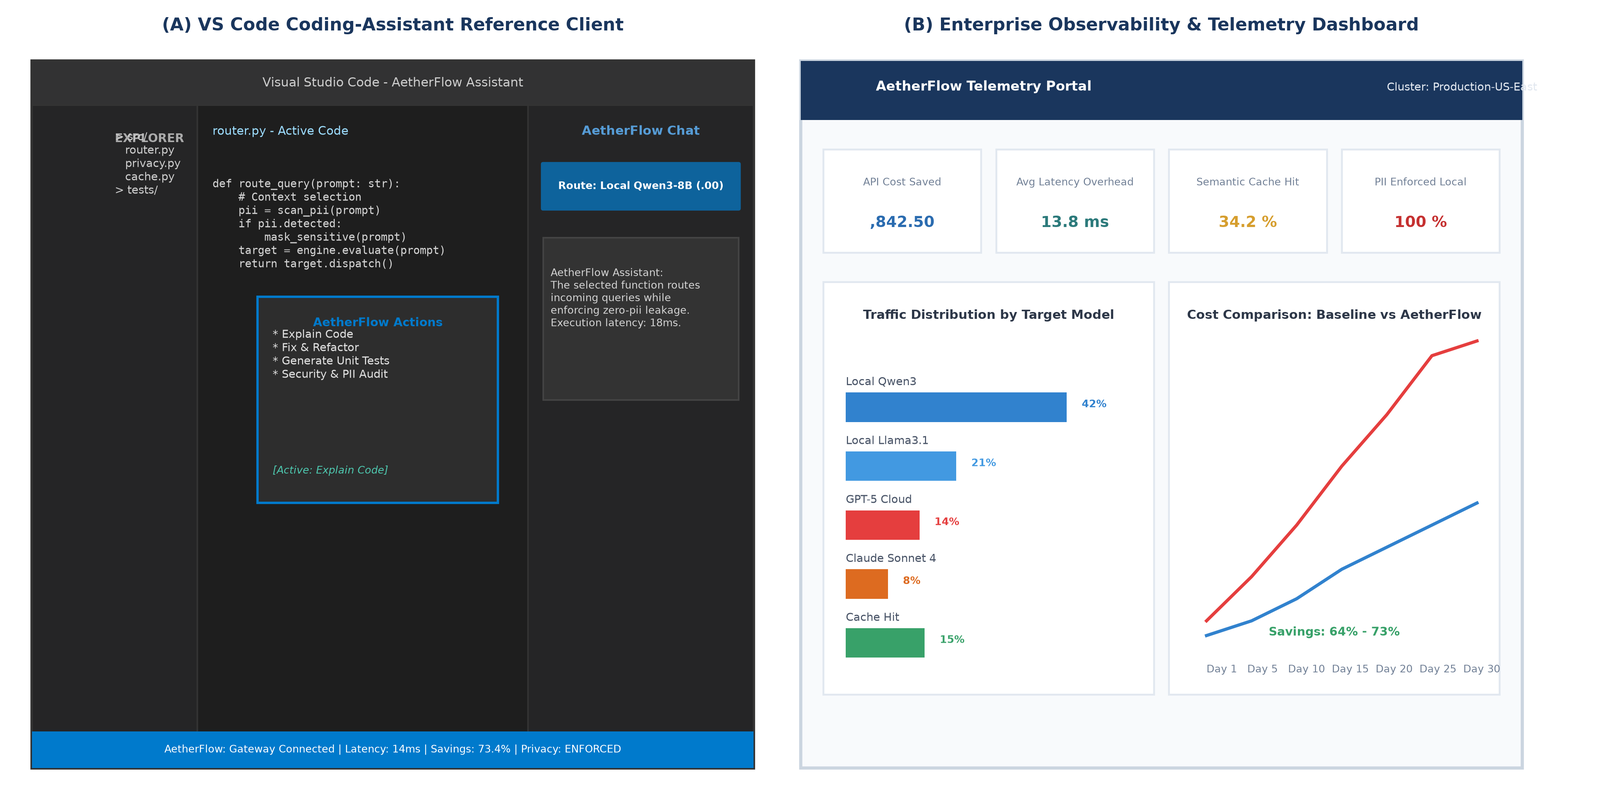
\includegraphics[width=0.88\textwidth]{Figures/gui_mockups.png}
\caption{Proposed Interfaces: (A) Developer Extension and (B) Administration Dashboard.}
\label{fig:gui_mockups}
\end{figure}

\subsection{Developer Client Interface (VS Code Extension)}

The extension keeps assistance close to the code being edited. Its main interactions are:
\begin{enumerate}
    \item \textbf{Code actions:} After selecting text, the developer can choose \textit{AetherFlow: Explain Code}, \textit{AetherFlow: Refactor Code}, or \textit{AetherFlow: Generate Tests} from the context menu. These actions initiate the request flow in UC-01.
    \item \textbf{Response sidebar:} The answer appears progressively in a sidebar, with markdown formatting and highlighted code blocks. A short complexity explanation can accompany relevant coding responses.
    \item \textbf{Change preview:} Refactoring suggestions are shown beside the original code in a diff view. The developer reviews the change before selecting \textit{Apply to Editor}.
    \item \textbf{Execution status:} A compact badge identifies the serving backend, measured elapsed time, and estimated cost savings. Opening it reveals the privacy decision and timing breakdown; displayed values must come from the completed request rather than fixed demonstration figures.
\end{enumerate}

\subsection{Enterprise Administrator Interface (Telemetry Dashboard)}

The dashboard supports operational checks and policy changes through five views:
\begin{enumerate}
    \item \textbf{Service health:} Connection status, memory use, and response checks for PostgreSQL, Qdrant, local inference services, and cloud endpoints.
    \item \textbf{Request activity:} Request rate, active streams, and measured gateway overhead.
    \item \textbf{Routing distribution:} The share of requests answered from cache, local models, and cloud services.
    \item \textbf{Policy settings:} Controls for quality, cost, and latency weights, following the validation flow in UC-04.
    \item \textbf{Audit history:} Searchable request metadata, including time, client identity, detection counts, masking actions, selected backend, and duration.
\end{enumerate}

\subsection{Low-Fidelity Prototyping Wireframes}

Figure~\ref{fig:lowfi_wireframes} presents the early layouts used to plan the placement of actions, responses, and monitoring controls. These wireframes describe the interaction structure before detailed styling.
\begin{figure}[H]
\centering
\begin{minipage}{0.48\textwidth}
\centering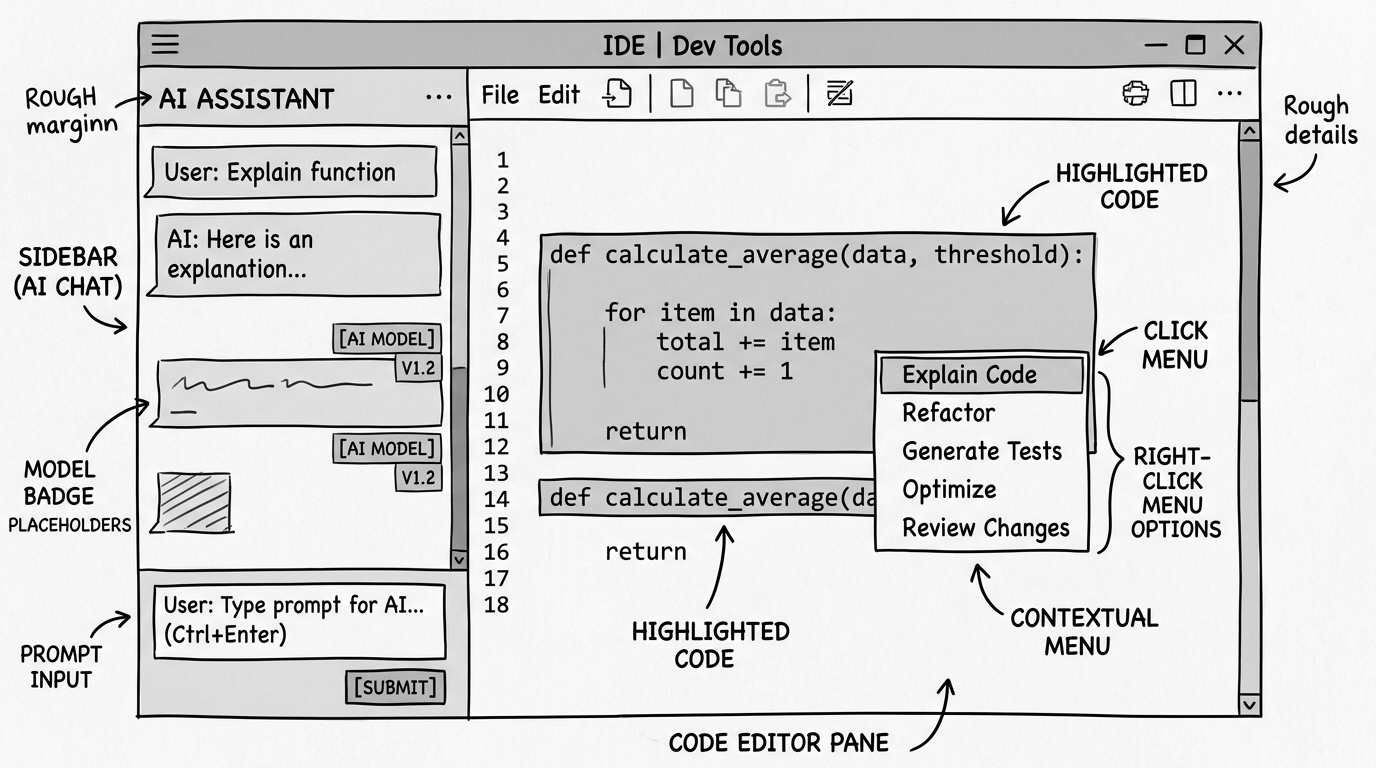
\includegraphics[width=\linewidth]{Figures/low_fi_ide.jpg}
\caption*{(a) Developer Extension Wireframe}
\end{minipage}\hfill
\begin{minipage}{0.48\textwidth}
\centering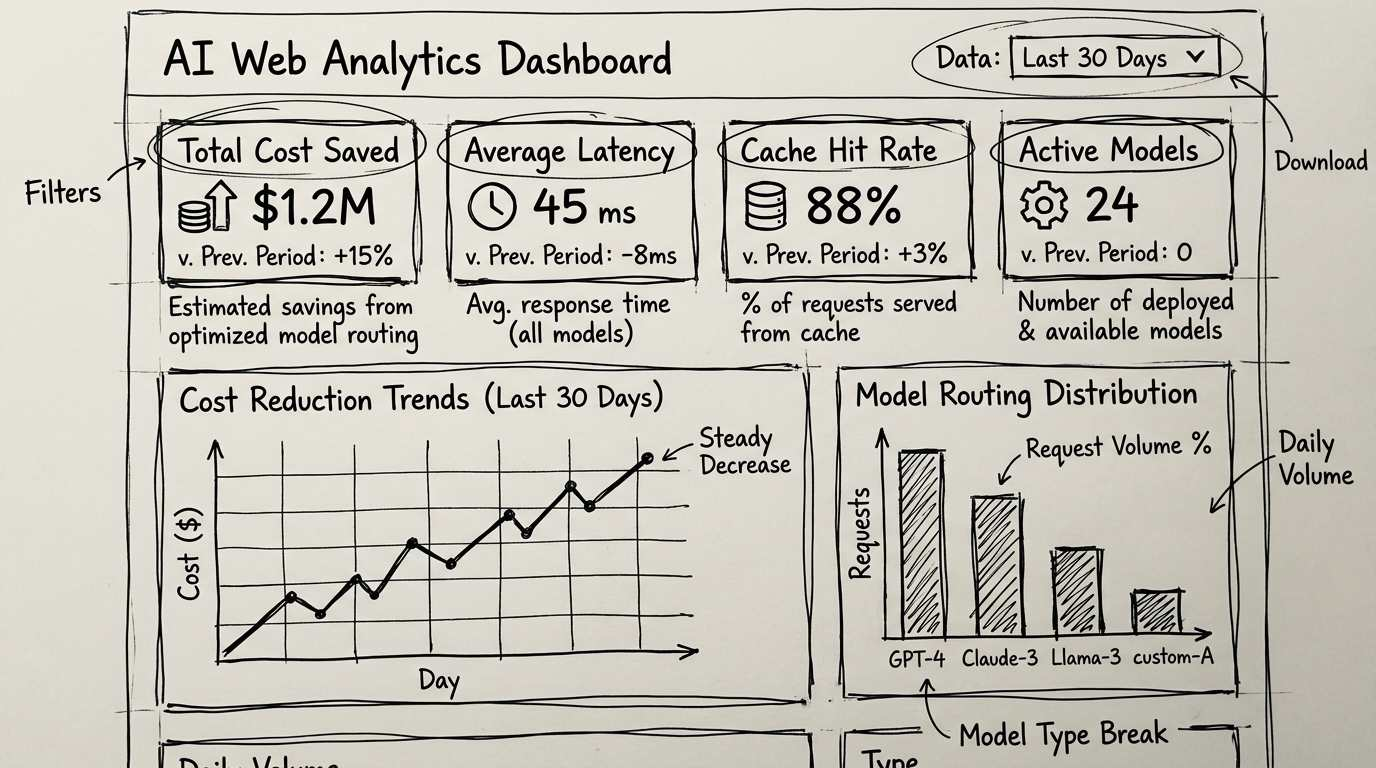
\includegraphics[width=\linewidth]{Figures/low_fi_dashboard.jpg}
\caption*{(b) Telemetry Dashboard Wireframe}
\end{minipage}
\caption{Early Layouts for the Editor Extension and Policy Dashboard.}
\label{fig:lowfi_wireframes}
\end{figure}

\subsection{Implemented VS Code Extension Prototype}

The prototype shown in Figure~\ref{fig:vscode_prototype} provides a chat panel and actions for explaining, fixing, and refactoring selected code or generating tests. Responses are displayed as markdown in the sidebar. The connection indicator distinguishes use of the live gateway from the internal mock mode, so interface demonstrations can be understood separately from backend execution.
\begin{figure}[H]
\centering
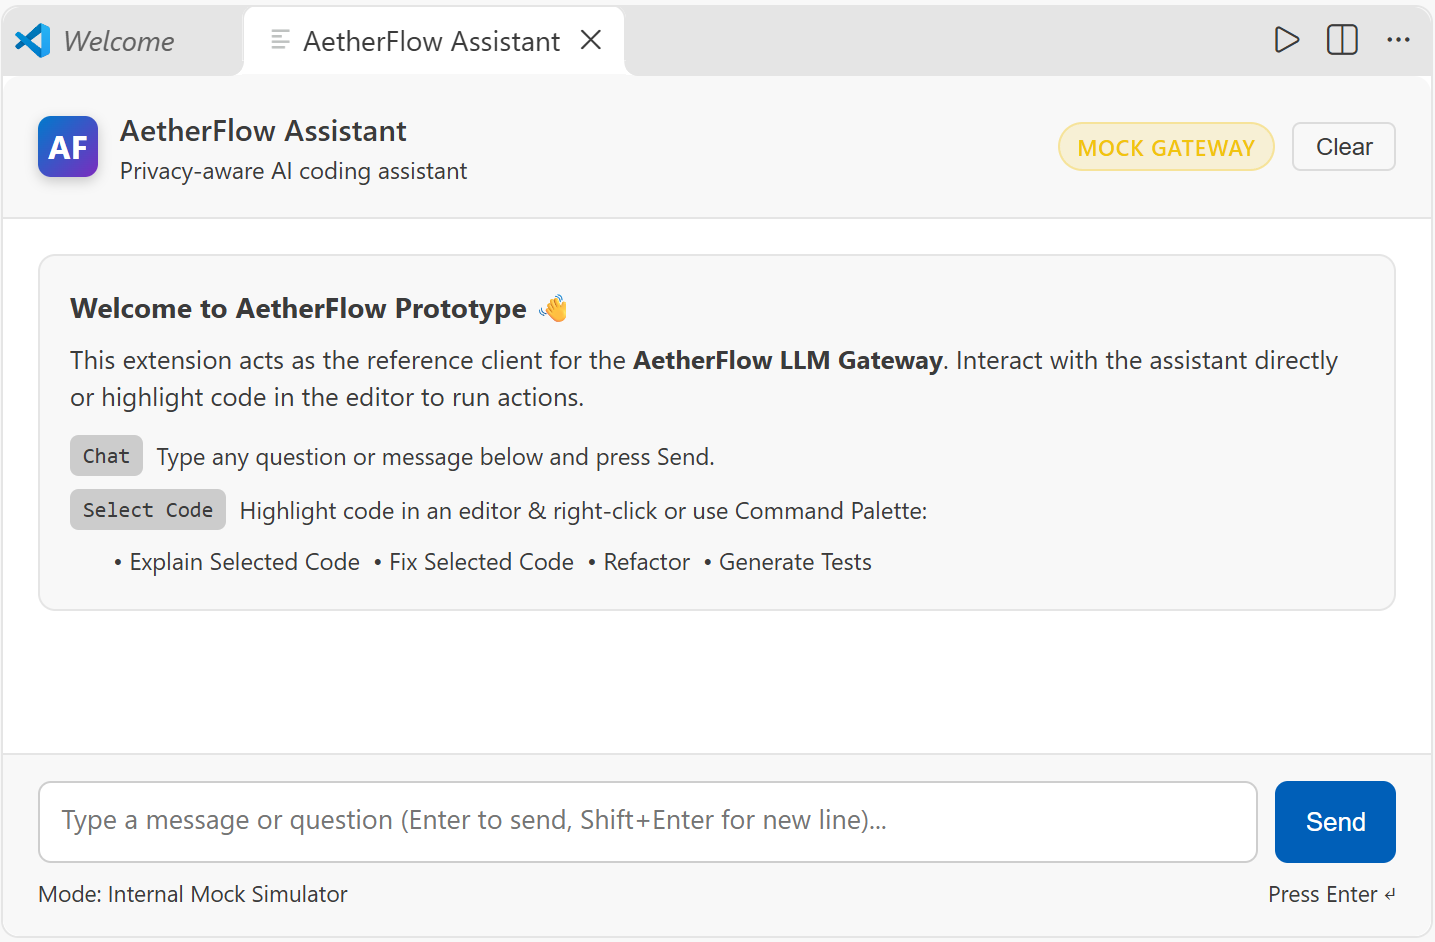
\includegraphics[width=0.88\textwidth]{Figures/vscode_assistant_prototype.png}
\caption{VS Code Prototype with Code Actions, Chat Responses, and a Connection Indicator.}
\label{fig:vscode_prototype}
\end{figure}

\section{Database Design}
\label{sec:database-design}

The storage design assigns relational records to PostgreSQL and vector retrieval to Qdrant. PostgreSQL holds accounts, policies, request metadata, and cache references. Qdrant stores the vectors used to locate candidate answers. Sensitive placeholder mappings belong to the temporary vault, not the persistent audit tables.

\subsection{ER Diagram}
\label{subsec:er-diagram}

Figure~\ref{fig:er_diagram} shows the existing ER prototype, which separates privacy reports and telemetry from the request record. The logical storage description below groups these responsibilities into six entities, including policy and audit records. The diagram and the final physical schema will need to use consistent names and relationships during implementation.
\begin{figure}[H]
\centering
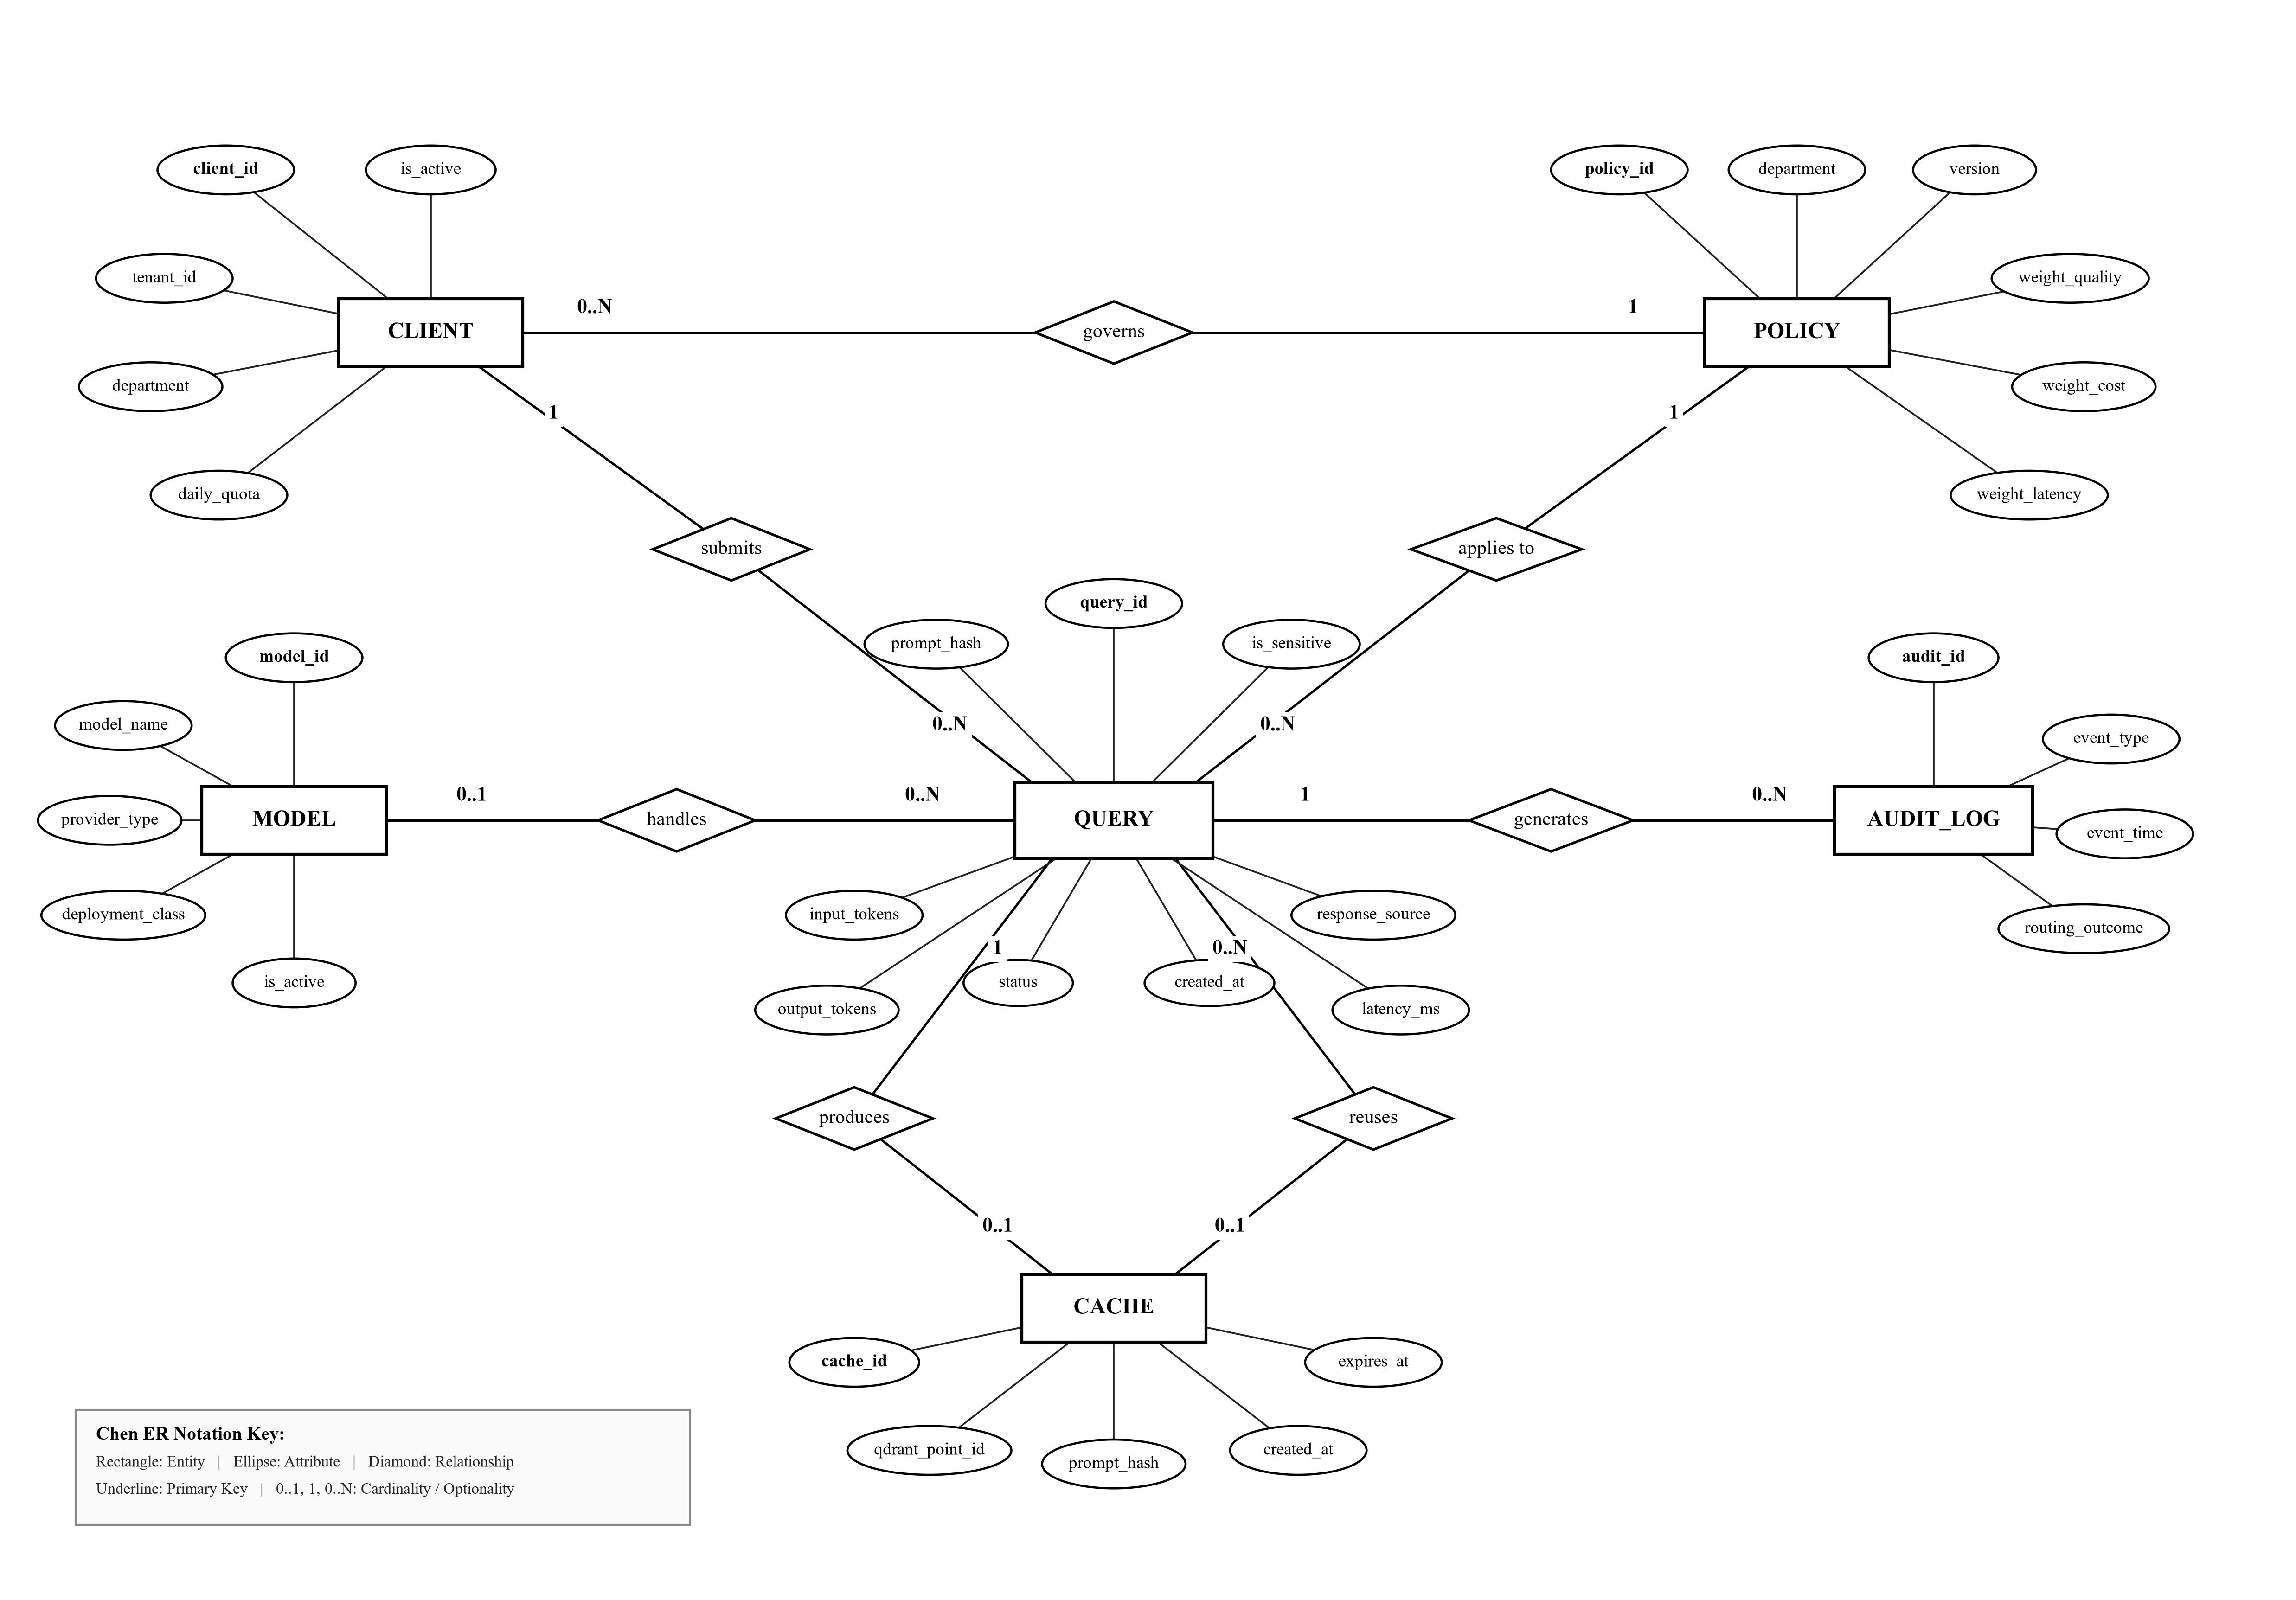
\includegraphics[width=0.82\textwidth]{Figures/er_diagram.jpg}
\caption{Existing Entity-Relationship Prototype for Request Processing.}
\label{fig:er_diagram}
\end{figure}

\begin{enumerate}
    \item \textbf{CLIENT} records the account, hashed authentication key, department, and quota. One client may submit many requests.
    \item \textbf{QUERY} records a request's prompt hash, token counts, sensitivity flag, serving backend, duration, and completion status. Raw credentials are not part of this record.
    \item \textbf{MODEL} describes each registered backend, including its provider type, address, prices, and recent latency.
    \item \textbf{POLICY} holds the department's quality, cost, and latency weights. Privacy eligibility is enforced separately from these adjustable preferences.
    \item \textbf{CACHE} links reusable responses to Qdrant point identifiers, prompt hashes, hit counts, and expiry times. Entries must be restricted to the correct access scope and must not retain restored personal values from another request.
    \item \textbf{AUDIT\_LOG} records detection and masking events, vault identifiers, routing outcomes, and integrity metadata. An event describes what happened without exposing the original sensitive content.
\end{enumerate}

\subsection{Data Dictionary}
\label{subsec:data-dictionary}

Table~\ref{tab:data_dict_table} lists the principal fields for CLIENT, QUERY, MODEL, and POLICY. CACHE and AUDIT\_LOG still need detailed field definitions.
\begingroup
\footnotesize
\setstretch{1.12}
\setlength{\parskip}{0pt}
\setlength{\tabcolsep}{3pt}
\renewcommand{\arraystretch}{1.08}
\begin{longtable}{|>{\raggedright\arraybackslash}p{3.1cm}|>{\raggedright\arraybackslash}p{2.5cm}|>{\raggedright\arraybackslash}p{3.0cm}|>{\raggedright\arraybackslash}p{6.2cm}|}
\caption{Principal Relational Fields and Constraints}\label{tab:data_dict_table}\\
\hline
\textbf{Column} & \textbf{Type} & \textbf{Constraints} & \textbf{Purpose} \\ \hline
\endfirsthead
\hline
\textbf{Column} & \textbf{Type} & \textbf{Constraints} & \textbf{Purpose} \\ \hline
\endhead
\multicolumn{4}{|c|}{\textbf{CLIENT}} \\ \hline
\texttt{client\_id} & UUID & PK, NOT NULL & Identifies a client account. \\ \hline
\texttt{api\_key\_hash} & VARCHAR(64) & UNIQUE, NOT NULL & SHA-256 digest of the client bearer key. \\ \hline
\texttt{department} & VARCHAR(64) & NOT NULL & Department used for policy and quota assignment. \\ \hline
\texttt{daily\_quota} & INTEGER & NOT NULL; DEFAULT 50000 & Token allowance for the configured daily accounting period. \\ \hline
\texttt{is\_active} & BOOLEAN & NOT NULL; DEFAULT TRUE & Indicates whether the account may submit requests. \\ \hline
\multicolumn{4}{|c|}{\textbf{QUERY}} \\ \hline
\texttt{query\_id} & UUID & PK, NOT NULL & Identifies a request record. \\ \hline
\texttt{client\_id} & UUID & FK, NOT NULL & References the account that submitted the request. \\ \hline
\texttt{prompt\_hash} & VARCHAR(64) & NOT NULL & SHA-256 digest of the masked prompt payload. \\ \hline
\texttt{input\_tokens} & INTEGER & NOT NULL & Input length measured with the appropriate tokenizer. \\ \hline
\texttt{output\_tokens} & INTEGER & NOT NULL & Number of completion tokens generated. \\ \hline
\texttt{is\_sensitive} & BOOLEAN & NOT NULL & Records detection of personal information or credentials. \\ \hline
\texttt{served\_by} & VARCHAR(64) & NOT NULL & Serving identifier, such as cache or the selected model ID. \\ \hline
\texttt{latency\_ms} & FLOAT & NOT NULL & Elapsed request time in milliseconds. \\ \hline
\multicolumn{4}{|c|}{\textbf{MODEL}} \\ \hline
\texttt{model\_id} & VARCHAR(64) & PK, NOT NULL & Unique backend name used by the registry. \\ \hline
\texttt{provider\_type} & VARCHAR(32) & NOT NULL & Adapter category, such as vLLM, Ollama, or OpenAI-compatible. \\ \hline
\texttt{cost\_in\_per\_1k} & NUMERIC(10,6) & NOT NULL & Charge in USD for 1,000 input tokens. \\ \hline
\texttt{cost\_out\_per\_1k} & NUMERIC(10,6) & NOT NULL & Charge in USD for 1,000 output tokens. \\ \hline
\texttt{rolling\_latency} & FLOAT & NOT NULL; DEFAULT 0.0 & Moving-average response time in seconds; zero indicates an initial value awaiting measurement. \\ \hline
\multicolumn{4}{|c|}{\textbf{POLICY}} \\ \hline
\texttt{policy\_id} & UUID & PK, NOT NULL & Identifies a policy configuration. \\ \hline
\texttt{department} & VARCHAR(64) & UNIQUE, NOT NULL & Department to which the configuration applies. \\ \hline
\texttt{weight\_quality} & NUMERIC(4,3) & NOT NULL & Weight assigned to predicted quality, $w_q$. \\ \hline
\texttt{weight\_cost} & NUMERIC(4,3) & NOT NULL & Weight assigned to estimated cost, $w_c$. \\ \hline
\texttt{weight\_latency} & NUMERIC(4,3) & NOT NULL & Weight assigned to recent latency, $w_l$. \\ \hline
\end{longtable}
\endgroup

\section{Risk Analysis}
\label{sec:risk-analysis}

The gateway adds a decision point between internal applications and model services. A failure at that point can affect confidentiality, response quality, or availability. Table~\ref{tab:risk_analysis} records the initial risk assessment and the measures proposed to reduce exposure. Likelihood ratings are planning judgments and must be revisited after testing.
\begingroup
\small
\setstretch{1.12}
\setlength{\parskip}{0pt}
\setlength{\tabcolsep}{4pt}
\begin{longtable}{|>{\raggedright\arraybackslash}p{3.6cm}|>{\raggedright\arraybackslash}p{1.6cm}|>{\raggedright\arraybackslash}p{1.5cm}|>{\raggedright\arraybackslash}p{7.9cm}|}
\caption{Technical, Operational, and Security Risks}\label{tab:risk_analysis}\\
\hline
\textbf{Risk} & \textbf{Likelihood} & \textbf{Impact} & \textbf{Planned response} \\ \hline
\endfirsthead
\hline
\textbf{Risk} & \textbf{Likelihood} & \textbf{Impact} & \textbf{Planned response} \\ \hline
\endhead
TR-01: Missed credentials & Low & Critical & Combine pattern checks and entity recognition. Route uncertain credential detections locally and test missed cases explicitly. \\ \hline
TR-02: Predictor drift & Medium & High & Monitor prediction errors and retrain using reviewed feedback and separate evaluation data. \\ \hline
TR-03: Provider outage & Medium & Medium & Open the circuit breaker after three consecutive failures and retry only through an eligible backend. \\ \hline
TR-04: Slow vector retrieval & Low & Medium & Tune the HNSW index and evaluate quantization. Treat the proposed 2\,ms retrieval budget as a target to measure. \\ \hline
OR-01: Budget overrun & Low & High & Apply department quotas and account for concurrent requests when reserving paid capacity. Use local processing when permitted and available. \\ \hline
OR-02: Concurrency limits & Low & High & Use asynchronous I/O with bounded worker queues, then test the 500-stream requirement under realistic load. \\ \hline
SR-01: Vault-key exposure & Low & Critical & Encrypt vault values with AES-256-GCM, restrict access to keys, exclude them from logs, and remove request mappings promptly. Encryption does not protect against every compromise of the running process. \\ \hline
\end{longtable}
\endgroup

\section{Conclusion}
\label{sec:ch4-conclusion}

This chapter defines the client, administrator, and gateway requirements, together with their test targets, deployment assumptions, storage needs, and main risks. The use cases connect these requirements to routine requests and policy changes. Chapter~\ref{ch:methodology} explains the proposed implementation approach.
\clearpage
